\documentclass[10pt]{article}
\usepackage[latin1]{inputenc}
\usepackage[english]{babel}
\usepackage{fancyvrb}
\usepackage[a4paper,margin=2cm]{geometry}
\usepackage{titlesec}
\usepackage{macrosens}
\usepackage{comment}
\usepackage{mathpazo}
\usepackage{ dsfont }
\usepackage{amsmath}
\usepackage{hyperref}


%\setlength{\parindent}{0pt}
\setlength{\parskip}{1ex}

%\titleformat{ command }[ shape ]{ format }{ label }{ sep }{ before }[ after ]
\titleformat{\section}{\large\bfseries}{Exercise \thesection.}{1ex}{}
%\titlespacing{\subsection}{0pt}{*2}{*1}

\renewcommand{\thesubsection}{\arabic{subsection}}

\titleformat{\subsection}[runin]{\normalsize\bfseries}{Q\thesubsection.}{1ex}{}
\titlespacing{\subsection}{0pt}{*2}{*1}


\specialcomment{correction}
{\begin{quote}
     \begin{em}
       \begin{tabular}{|p{\linewidth}|}\hline
      % \rule[-2.7ex]{0.6pt}{1.2em}\noindent\makebox[\linewidth]{\rule{\linewidth}{0.6pt}}
     % \centering
        \begin{minipage}{0.9\linewidth}
}{
        \end{minipage}
       \\\hline
         \end{tabular}
%\\ \rule[0.0ex]{0.6pt}{1.2em}\noindent\makebox[\linewidth]{\rule{\linewidth}{0.6pt}}
       \end{em}
  \end{quote}
}

\newcommand{\smallcorr}[1]{\hfill\emph{\begin{tabular}[c]{|l|}\hline #1\\\hline\end{tabular}}}
% 2 lines below to comment to get the correction
\renewcommand{\smallcorr}[1]{}
%\excludecomment{correction}

\begin{document}

\pagestyle{empty}

\noindent
\textbf{IST Austria} \hfill %\textbf{Polytech Grenoble} \\
\textbf{Numerical Algorithms} \hfill \textbf{Spring 2017}



%\lstset{
%  language=Algo,
%  basicstyle=\sffamily,
%  columns=fullflexible,
%  mathescape
%}

\begin{center}
{\large\textbf{Homework 2: Linear systems}}\\
Due Wednesday, March 15.
\end{center}

\noindent\makebox[\linewidth]{\rule{\linewidth}{0.6pt}}
 
\section*{Instructions}

\begin{itemize}
\item The assignments must be dropped off in the T.A. mail box: Office Building West, 2nd floor, left of the stairs, top-left box (Camille Schreck), or sent to me by email. The deadline is March 14  at midnight.
\item The assignments may be handwritten or typed. You can code in any programming language. The code itself will not be reviewed. 
\item The textbook is \emph{Numerical Algorithms} from Justin Solomon.\\ \url{https://people.csail.mit.edu/jsolomon/share/book/numerical_book.pdf}.
\item The textbook do not talk about Jacobi and Gauss-Seidel methods. You can also look up the Wikipedia pages on the subject if you need more details.\\
  \url{https://en.wikipedia.org/wiki/Jacobi's_method}\\
  \url{https://en.wikipedia.org/wiki/Gauss-Seidel_method}
  
\end{itemize}



\noindent\makebox[\linewidth]{\rule{\linewidth}{0.6pt}}

\section*{Exercise 1: Condition number and eigenvalues \normalsize \textnormal(50 points)}

\subsection{} Let's call $cond(A) = ||A||\;||A^{-1}||$ the condition number of the matrix $A \in \mathds{R}^{n\times n}$, and $\sigma_{min}$  and $\sigma_{max}$ are respectively the largest and smallest eigenvalues of $A$ (in absolute value). 
Prove that the $cond(A) \leq \frac{|\sigma_{max}|}{|\sigma_{min}|}$.

\emph{Hint: you may want to look at the singular value decomposition of $A$.}

\begin{correction}

\end{correction}

\subsection{} You are given a linear system $A\mathbf{x}=\mathbf{b}$ with condition number $cond(A)=C$. What is the condition number of the least squares system $A^TA\mathbf{x}=A^T\mathbf{b}$, in terms of $C$? What does this tell you about the difficulty to accurately solve a least-squares problem relative to the original system?

\begin{correction}

\end{correction}

\subsection{} You are given a matrix $A = 
\left(\begin{matrix}
u_1 & v_1\\
u_2 & v_2
\end{matrix}\right)$.
\begin{itemize}
\item Compute its characteristic polynomial $det(A-\lambda I)$, where $I$ is the identity matrix, and $\lambda$ is an eigenvalue of $A$. Express it using the trace $T$ and determiant $D$ of $A$.
\item The eigenvalues of a matrices are the solutions of $det(A-\lambda I) = 0$. Express them in terms of $T$ and $D$.
\item Assuming the eigenvalues are real, express the condition number in terms of $T$ and $D$. When is it maximal and when is it minimal ?
\item \textit{\textbf{Bonus:} } How does the condition number relate to the angle between the two vectors $\mathbf u = (u_1,u_2,0)^T$ and $\mathbf v = (v_1,v_2,0)^T$.
  %Derive an explicit formula relating the condition number of $A$ to the angle between the two vectors $\mathbf u = (u_1,u_2,1)^T$ and $\mathbf v = (v_1,v_2,1)^T$.
  \end{itemize}
%Use this to solve for the maximum and minimum eigenvalues, and compute the condition number of $A$. 
%Derive an explicit formula relating the condition number of $A$ to the angle between the two vectors $\mathbf u = (u_1,u_2,1)^T$ and $\mathbf v = (v_1,v_2,1)^T$.

\begin{correction}

\end{correction}


\section*{Exercise 2: iterative methods \normalsize \textnormal(50 points)}

In class, we discussed {\em Jacobi iteration} and {\em Gauss-Seidel iteration}, two splitting-based methods for solving a linear system. Implement both of these algorithms in whatever programming language you like, and we will and test them in the following problems.

A vector $\mathbf x \in \mathds{R}^{10}$ represents some function on the nodes of the graph below. 
\begin{figure}[h!]
\centering
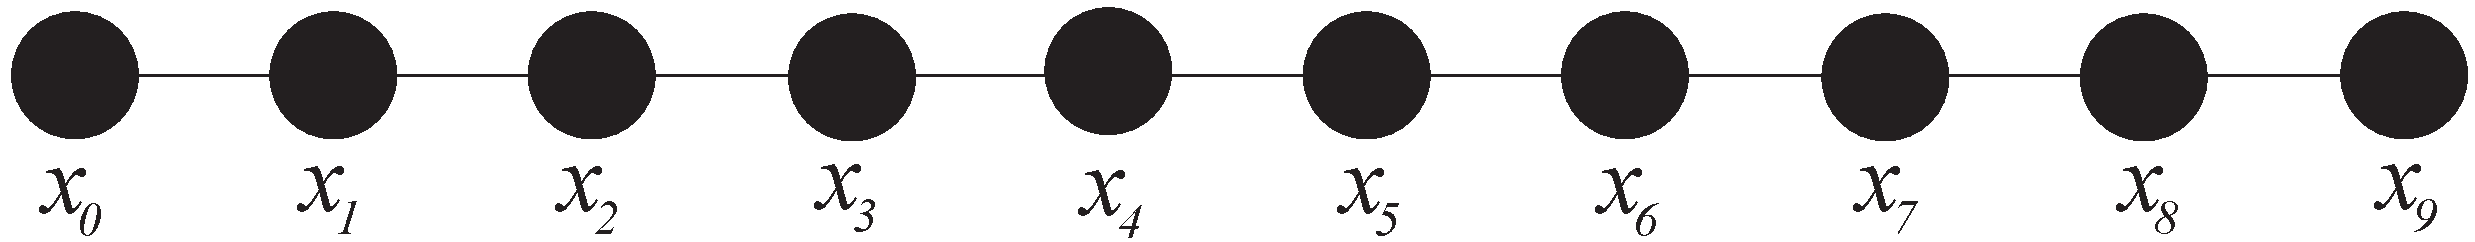
\includegraphics[width=0.8\textwidth]{graph.pdf}
\end{figure}

A linear system $A\mathbf{x}=\mathbf{b}$ with
\begin{equation*}
A = 
\left(\begin{matrix}
1& -1& 0& 0& 0& 0& 0& 0& 0& 0\\
-1& 2& -1& 0& 0& 0& 0& 0& 0& 0\\
0& -1& 2& -1& 0& 0& 0& 0& 0& 0\\
0& 0& -1& 2& -1& 0& 0& 0& 0& 0\\
0& 0& 0& -1& 2& -1& 0& 0& 0& 0\\
0& 0& 0& 0& -1& 2& -1& 0& 0& 0\\
0& 0& 0& 0& 0& -1& 2& -1& 0& 0\\
0& 0& 0& 0& 0& 0& -1& 2& -1& 0\\
0& 0& 0& 0& 0& 0& 0& -1& 2& -1\\
0& 0& 0& 0& 0& 0& 0&  0&-1& 1\\
\end{matrix} \right),  \hspace{1cm} 
\mathbf{x} = \left(\begin{matrix}
x_0\\
x_1\\
x_2\\
x_3\\
x_4\\
x_5\\
x_6\\
x_7\\
x_8\\
x_9
\end{matrix} \right), \hspace{1cm} \text{and} \hspace{1cm}
\mathbf{b} = \left(\begin{matrix}
0\\
0\\
0\\
0\\
0\\
0\\
0\\
0\\
0\\
0
\end{matrix} \right)
\end{equation*}
constrains each $x_i$ to be the average of its neighbors. (Please verify this for yourself.)

\subsection{} Starting with an initial guess $\mathbf{x}=(9,1,7,3,5,9,1,7,3,5)^T$, solve this system with Jacobi iteration, Gauss-Seidel iteration ordered from $x_0 \to x_9$, and Gauss-Seidel iteration ordered from $x_9 \to x_0$. Record the solution $\mathbf{x}$ and plot the convergence rate for each method. Explain any obvious differences you may find.

\subsection{} What is the theoretical solution $\mathbf{x}$? 

\subsection{} Discuss the stability of this linear system. Use whatever arguments or tools you like.

\section*{Exercise 3: More iterative methods \normalsize \textnormal(xx points)}

Next, let's work with the modified system $A\mathbf{x}=\mathbf{b}$ with
\begin{equation*}
A = 
\left(\begin{matrix}
-1& 2& -1& 0& 0& 0& 0& 0& 0& 0\\
0& -1& 2& -1& 0& 0& 0& 0& 0& 0\\
0& 0& -1& 2& -1& 0& 0& 0& 0& 0\\
0& 0& 0& -1& 2& -1& 0& 0& 0& 0\\
0& 0& 0& 0& -1& 2& -1& 0& 0& 0\\
0& 0& 0& 0& 0& -1& 2& -1& 0& 0\\
0& 0& 0& 0& 0& 0& -1& 2& -1& 0\\
0& 0& 0& 0& 0& 0& 0& -1& 2& -1\\
0& 0& 0& 0& 0& 0& 0& 0& -1& 1\\
0& 0& 0& 0& 0& 0& 0& 0& 0& 1\\
\end{matrix} \right),  \hspace{1cm} 
\mathbf{x} = \left(\begin{matrix}
x_0\\
x_1\\
x_2\\
x_3\\
x_4\\
x_5\\
x_6\\
x_7\\
x_8\\
x_9
\end{matrix} \right), \hspace{1cm} \text{and} \hspace{1cm}
\mathbf{b} = \left(\begin{matrix}
0\\
0\\
0\\
0\\
0\\
0\\
0\\
0\\
0\\
0
\end{matrix} \right)
\end{equation*}

\subsection{} If the previous system set each $x_i$ to the average of its neighbors, what does this system do?

\subsection{} Starting with an initial guess $\mathbf{x}=(9,1,7,3,5,9,1,7,3,5)^T$, solve this system with Jacobi iteration, Gauss-Seidel iteration ordered from $x_0 \to x_9$, and Gauss-Seidel iteration ordered from $x_9 \to x_0$. Record the solution $\mathbf{x}$ and plot the convergence rate for each method. Explain any obvious differences you may find.

\subsection{} What is the theoretical solution $\mathbf{x}$? 

\subsection{} Discuss the stability of this linear system. Use whatever arguments or tools you like.

\iffalse
\subsection{} 

\subsection{} Let's choose:
$$ A = 
\left(\begin{matrix}
4& 0.6& 0& 0& 0\\
      0.6& 8& 0.2 & 0& 0\\
      0& 0.2& 15& 0.1& 0\\
    0& 0& 0.1& 16& 0\\
    0& 0& 0& 0& 42;

\end{matrix} \right)\hspace{1cm} \text{and} \hspace{1cm}
b = \left(\begin{matrix}
5.2\\
17.2\\
45.8\\
64.3\\
210
\end{matrix} \right)
$$

Find $x$ such that $Ax = b$ using Jacobi method and then Gauss-Seidel. Do both methods converge ? How many iterations do you need ? What is the error at the end ?

\subsection{} Now let's choose:
$$ A = 
\left(\begin{matrix}
2& -1& 0& 0& 1\\
    -1& 2& -1& 0& 0\\
    0& -1& 2& -1& 0\\
    0& 0& -1& 2& -1\\
    1& 0& 0& -1& 2
\end{matrix} \right)\hspace{1cm} \text{and} \hspace{1cm}
b = \left(\begin{matrix}
5\\
0\\
0\\
0\\
7
\end{matrix} \right)
$$
Same questions as before.\\
The exact solution is:
$$ x = \left(\begin{matrix}
1\\
2\\
3\\
4\\
5
\end{matrix} \right)
$$
Plot the backward and forward error for the Gauss-Seidel method:
\fi


\end{document}
